%% This is an example first chapter.  You should put chapter/appendix that you
%% write into a separate file, and add a line \include{yourfilename} to
%% main.tex, where `yourfilename.tex' is the name of the chapter/appendix file.
%% You can process specific files by typing their names in at the 
%% \files=
%% prompt when you run the file main.tex through LaTeX.
\chapter{\hlc[cyan]{Introduction}}

\section{\hlc[cyan]{Research Problems, Questions, \& Contributions}} \label{sec:questions}

Over the past two decades satellite-based remote observation has blossomed. We have seen a rapid increase in the number of \acp{eos} in orbit \cite{belwardWhoLaunchedWhat2015}, significant improvements in their capabilities \cite{jensenRemoteSensingEnvironment2006}, and much greater availability of the data that they produce \cite{borowitzOpenSpaceGlobal2017}. The diversity of designing, launching, and operating organizations has also expanded. \acp{eos} are no longer the sole province of the militaries and space agencies of a handful of nations. Private companies, universities, and new space nations have all joined the field [cite]. These trends have occurred as part of broader technological and societal trends of increasing data availability, computational power, modeling ability, and technical knowledge. 

This is remarkable because, despite some efforts in previous decades \cite{lightWarfareWelfareDefense2005}, \ac{eo} data has been largely used only by governments and academics for military and scientific purposes, with the latter focused on understanding and predicting environmental phenomena. Large corporations and \acp{ngo} have recently been conducting their own analyses (as seen in the growing industry of climate consultants \cite{cohenTop10Climate2011}), but these have required significant expertise and resources, and the results have sadly been mostly unavailable to the broader public.

The proliferation of \ac{eo} (and other) data, and in particular the improvements in spatial and temporal resolution, have opened the door for new kinds of applications. Among these are those at smaller spatial scales and shorter durations. Where historical civilian applications focused on how the environments of nations or continents changed over the course of years or decades, we can increasingly ask questions of on a much more human scale: neighborhoods, towns, and even individual buildings. Obviously new methods must be developed for such applications. Models that work well on a global scale often do not function at the scale of a few blocks. The our understanding of context and our ethical framework must also adapt. No longer are we asking questions about "agriculture in Canada" or "the Brazilian Amazon." We are now asking questions about particular farms, ranches, homes, and communities. The residents of this places should have not just a say, but significant involvement in how this data is used to impact their lives. This moves us from the fields that have traditionally dominated \ac{eo} (earth science, aerospace engineering, physics, etc.) to those that specialize in operating at such scales (urban planning, anthropology, community organizing, etc.). This poses a problem, as most of those who seek to apply \ac{eo} data in these new domains come from the former background, not the latter. They may not understand the expertise, history, and ethics needed to operate on these scales and may seek to continue to apply their traditional techniques. This risks not just failing in their own eyes, but also inflicting collateral damage on the communities that they are seeking to help.

[consider adding text about sustainable development here] Along with this increase in supply of data and analysis capabilities, there has been a corresponding increase in demand, particularly for sustainable development applications. Where previously the fields of environmental conservation and human welfare / economic development were handled largely separately, sustainable development treats this domains as jointly bound in complex systems. 

There is a thus real need for:

\begin{enumerate}[label=\emph{\alph*},itemsep=0pt,parsep=0pt]
	\item{Developing models that can be used at smaller geographic and temporal scales. This includes making remote observation data not just available but accessible to a broader audience by developing data products that are relevant to everyday individuals.}
	\item{Bridging the traditional \ac{eo} fields with the traditional community planning and social fields. This will enable linking the \ac{eo}-supported environmental modeling with the societal impact of a changing environment as well as more direct monitoring of human society with \ac{eo} data.}
	\item{Building or adapting frameworks that community participation and collaboration in the use of \ac{eo} data. This includes putting policy and sensor design decision-making in the hands of a broader population.}
\end{enumerate}

This work aims to demonstrate the viability of a particular methodology for advancing towards each of these three goals. To that end, this work centers on exploring the efficacy and difficulties of \textbf{\textit{collaboratively developing}} a \textbf{\textit{systems-architecture-informed}}, multidisciplinary \textbf{\textit{\ac{gis} \ac{dss}}} for \textbf{\textit{sustainable development}} applications that makes significant use of \textbf{\textit{remote observation data}}. This involves expanding and codifying the previously proposed \ac{evdt} Modeling Framework  for combining \ac{eo} and other types of data to inform decision-making in complex socio-environmental systems, particularly those pertaining to sustainable development \cite{reidCombiningSocialEnvironmental2019}. Specifically this work will seek to address the following numbered \textbf{Research Questions} via the listed lettered \textbf{Research Deliverables}. The chapters that primarily address each deliverable are noted.

\begin{enumerate}[itemsep=0pt,parsep=0pt]
	\item{What aspects of systems architecture (and systems engineering in general) are relevant and useful for approaching issues of sustainability in complex \ac{sets}? In particular, how can they be adapted using techniques from collaborative planning theory and other critical approaches to enable avoid the technocratic excesses of the past?}
	\begin{enumerate}[label=\emph{\alph*},itemsep=0pt,parsep=0pt]
		\item{A critical analysis of systems engineering, \ac{gis}, and the other technical fields relied upon in this work [Chapter \ref{ch:theory}] }
		\item{A proposed framework for applying systems engineering for sustainable development in an anticolonialist manner} [Chapter \ref{ch:evdt}]
	\end{enumerate}
	\item{What are the sustainability benefits of collaborative development of \acp{dss} using the \ac{evdt} Modeling Framework in complex \ac{sets}?}
	\begin{enumerate}[label=\emph{\alph*},itemsep=0pt,parsep=0pt]
		\item{System architecture analyses of each of the case studies [Chapters \ref{ch:mangroves} \& \ref{ch:vida}]} 
		\item{Development of an \ac{evdt}-based \ac{dss} for each of the case studies [Chapters \ref{ch:mangroves} \& \ref{ch:vida}]} 
		\item{An interview-based assessment of the development process and usefulness of each \ac{dss} [Chapters \ref{ch:mangroves} \& \ref{ch:vida}]} 
	\end{enumerate}
	\item{What steps are necessary to establish \ac{evdt} as a continually development framework, a community of practice, and a growing code repository?}
	\begin{enumerate}[label=\emph{\alph*},itemsep=0pt,parsep=0pt]
		\item{An assessment of lessons learned from these \ac{dss} development processes [Chapter \ref{ch:discussion}]} 
		\item{An outline of potential future \ac{evdt} refinement and extension, such as using \ac{evdt} to inform the development of future \ac{eo} systems that are better designed for particular application contexts [Chapter \ref{ch:discussion}]}
	\end{enumerate}
\end{enumerate}

It should be noted that these questions are the overarching questions for this thesis. Each case study project is done in collaboration with local partners and is aimed at providing practical benefits. As a result, each case study \ac{dss} has its own specific objectives.

A quick note on the user of first person pronouns in this piece. The word `I' will obviously refer to the author, Jack Reid, and will be commonly used when describing work that I have done, arguments that I am asserting, etc. That said, the \ac{evdt} Framework and its various implementations, including the Vida \ac{dss}, were not solo projects but instead involved multiple contributors, both inside the Space Enabled Research Group and outside of it. Thus when I use `we' when talking about \ac{evdt} I will be referring to this collection of individuals. Additionally, sometimes I will use `we' to refer to the Space Enabled Research Group, particularly when discussing our group's set of methodologies and principles. Finally, on occasion, I may use `we' in the general humanistic sense. I will strive to make in which sense I am using `we' clear in context.

\section{\hlc[cyan]{Framing}}

This piece is fundamentally about modeling, in particular, multidisciplinary modeling, and how modeling can inform actual action. Now individual models are inherently simplifications, intentional or otherwise, aimed at accomplishing a goal. They are metaphors for how the world really works, intended to enhance human faculties and focus our intention. Now the problem with such metaphors is that, as Elizabeth Ostrom puts it, "Relying on metaphors as the foundation for policy advice can lead to results substantially different from those presumed to be likely... One can get trapped in one's own intellectual web. When years have been spent in the development of a theory with considerable power and elegance, analysts obviously will want to apply this tool to as many situations as possible... Confusing a model with the theory of which it is one representation can limit applicability still further" \cite{ostromGoverningCommonsEvolution2015}. 

This is of course only compounded when multiple models from different domains are strung together, as will be described later. We must accordingly be focused on maintaining intellectual humility and avoid catching ourself in our own web. Fortunately, such interdisciplinary humility is a key principle of the Space Enabled Research Group of which I am a part. We choose to practice a certain "theoretical pluralism" \cite{turkleEmpathyDiariesMemoir2021} in our methods, learning from those of different fields and not assuming that, merely because we have chose a certain approach, it is the only or the best possible approach.

In addition to our theoretical pluralism, we must also practice a humility in application. Much of our sustainable development work takes place in communities or even countries to which we are outsiders. There is a real danger that we rush in and prescribe the wrong solution to a problem that the community faces or misidentify the problem altogether. We could even to identify a problem were none, in fact exists, pathologizing the normal and natural, as the Victorian England medical profession did to women \cite{duffinConspicuousConsumptiveWoman2012}. 

As is described further later, we strive to avoid this by allowing actual community members to identify the problem; by speaking with multiple community members to garner different perspectives; and, when possible, spending time in the community ourselves. These latter two components are key, because even the member or leader of a community may be afflicted with significant misapprehensions about aspects of their own community, particularly of those who are seen inferior due to economic class, race, gender, education, or some other marker. Jane Jacob's described such a phenomena vividly in her classic text, showing that even a statistics-driven urban planner could, \textit{in contradiction to his own statistics}, let his prejudices determine his perspective of the North End of Boston. \textit{The Death and Life of Great American Cities} \cite{jacobsDeathLifeGreat2016}:

\blockquote{Consider, for example the orthodox planning reaction to a district called the North End in Boston. This is an old, low-rent area merging into the heavy industry of the waterfront, and it is officially considered Boston's worst slum and civic shame... When I saw the North End again in 1959, I was amazed at the change. Dozens and dozens of buildings had been rehabilitated... The general street atmosphere of buoyancy, friendliness, and good health was so infectious that I began asking directions of people just for the fun of getting in on some talk. I had seen a lot of Boston in the past couple of days, most of it sorely distressing, and this struck me, with relief, as the healthiest place in the city... I called a Boston planner I know.

"Why in the world are you down in the North End?" he said, "That's a slum!... It has among the lowest delinquency, disease, and infant mortality rates in the city. It has has the lowest ratio of rent to income in the city... the child population is just above average for the city, on the nose. The death rate is low, 8.8 per thousand, against the average city rate of 11.2. The TB death rate is very low, less than 1 per ten thousand, [I] can't understand it, it's lower even than Brookline's. In the old days the North End used to be the city's worst spot for tuberculosis, but all that has changed. Well, they must be strong people. Of course it's a terrible slum."

"You should have more slums like this," I said.} 

By speaking with different members of a community and striving to maintain an open mind about the communities that we work with, we can hope to avoid making a similar mistake.

\section{\hlc[cyan]{Space Enabled Principles}}

The mission of the Space Enabled research group is \textit{to advance justice in Earth's complex systems using designs enabled by space.} By "designs enabled by space," we mean primarily six types of space technology that support societal needs: satellite earth observation, satellite communication, satellite positioning, microgravity research, technology transfer, and the inspiration we derive from space research and education. By "advance justice in Earth's complex systems," we mean a combination of social justice (e.g. antiracism and anticolonialism) and sustainable development\footnote{Space Enabled usually refers to the \ac{un} \acp{sdg} to explain sustainable development, but a more detailed discussion of that term is provided in Section \ref{sec:sustain}.}. Fulfilling this mission is not just an issue of research topics but also of methodology, as "the master's tools will never dismantle the master's house" \cite{lordeMasterToolsWill1984}. Our methods are thus of necessity multidisciplinary, drawing from at least six disciplines: design thinking, art, social science, complex systems, satellite engineering and data science. Our work, unlike the long, problematic history of systems engineering and development (see Section \ref{sec:critiques}), is heavily dependent on local partnerships and collaborations with multilateral organizations, national and local governments, non-profits, entrepreneurial firms, local researchers, and other community leaders, both formal and informal. These collaborators guide the research directions and objectives, as well as participating as fully as they desire in each step of the research process.

It should be noted that pursuing these principles is forever a process of improvement. Large sections of Chapter \ref{ch:theory} of this thesis are aimed as such self-critique and improvement. 

\section{\hlc[cyan]{Methodology Summary \& Structure of Thesis}}

The structure of this thesis, along with the connections of each component to the Research Deliverables (RDs), is summarized in Figure \ref{fig:structure} below.

Chapter \ref{ch:theory} presents the theoretical underpinnings of this work, motivation for its pursuit, and various critical analysis based on literature reviews. The last of these will constitute Research Deliverable 1a and are primarily contained in Section \ref{sec:critiques} but are reliant upon the earlier sections. This will serve to expand upon the research problems introduced in Section \ref{sec:questions} and justify the novelty of the research contributions in the subsequent chapters. 

Chapter \ref{ch:evdt} provides details on the \ac{evdt} Framework, its intended applications, and its novelty. This constitutes Deliverable 1b. 

Chapters \ref{ch:mangroves} and \ref{ch:vida} contain the primary experimental components of this work in response to Research Question 2. This takes the form of the development and evaluation of \ac{evdt} \acp{dss} for two primary applications: (1) mangrove forest management and conservation in the state of Rio de Janeiro, Brazil [Chapter \ref{ch:mangroves}]; and (2) coronavirus response in six metropolitan areas across Angola, Brazil, Chile, Indonesia, Mexico, and the United States [Chapter \ref{ch:vida}]. In both cases, the methodology involves the application the \ac{saf} \cite{maierArtSystemsArchitecting2009, crawleySystemArchitectureStrategy2015} an approach that has been previously adapted from the aerospace engineering discipline by Prof. Wood for use in sociotechnical systems \cite{pfotenhauerArchitectingComplexInternational2016}. This includes using stakeholder mapping and network analysis to inform the design of the \ac{dss} in question as well as fulfilling Deliverable 2a. Other components of the methodology taken in this work are developing the \ac{dss} through an iterative and collaborative process with specific stakeholders; pursuing targeted, related analyses, such as on the value of certain ecosystem services, the value of remote sensing information, and human responses to various policies; and evaluating the usefulness of both the \ac{dss} and the development process through interviews, workshops, and other feedback mechanisms. 

Chapter \ref{ch:discussion} contains discussion on both applications and lessons learned. This will serve to address Research Question 3, lessons learned will be identified from the two case studies and from other \ac{evdt} projects undertaken by fellow students and I. These will be used to lay out a future development path for \ac{evdt} will be laid out.

Chapter \ref{ch:conclusion} provides a short conclusion summarizing this thesis.

\clearpage
\begin{landscape}
\begin{figure}[t]
	\centering
	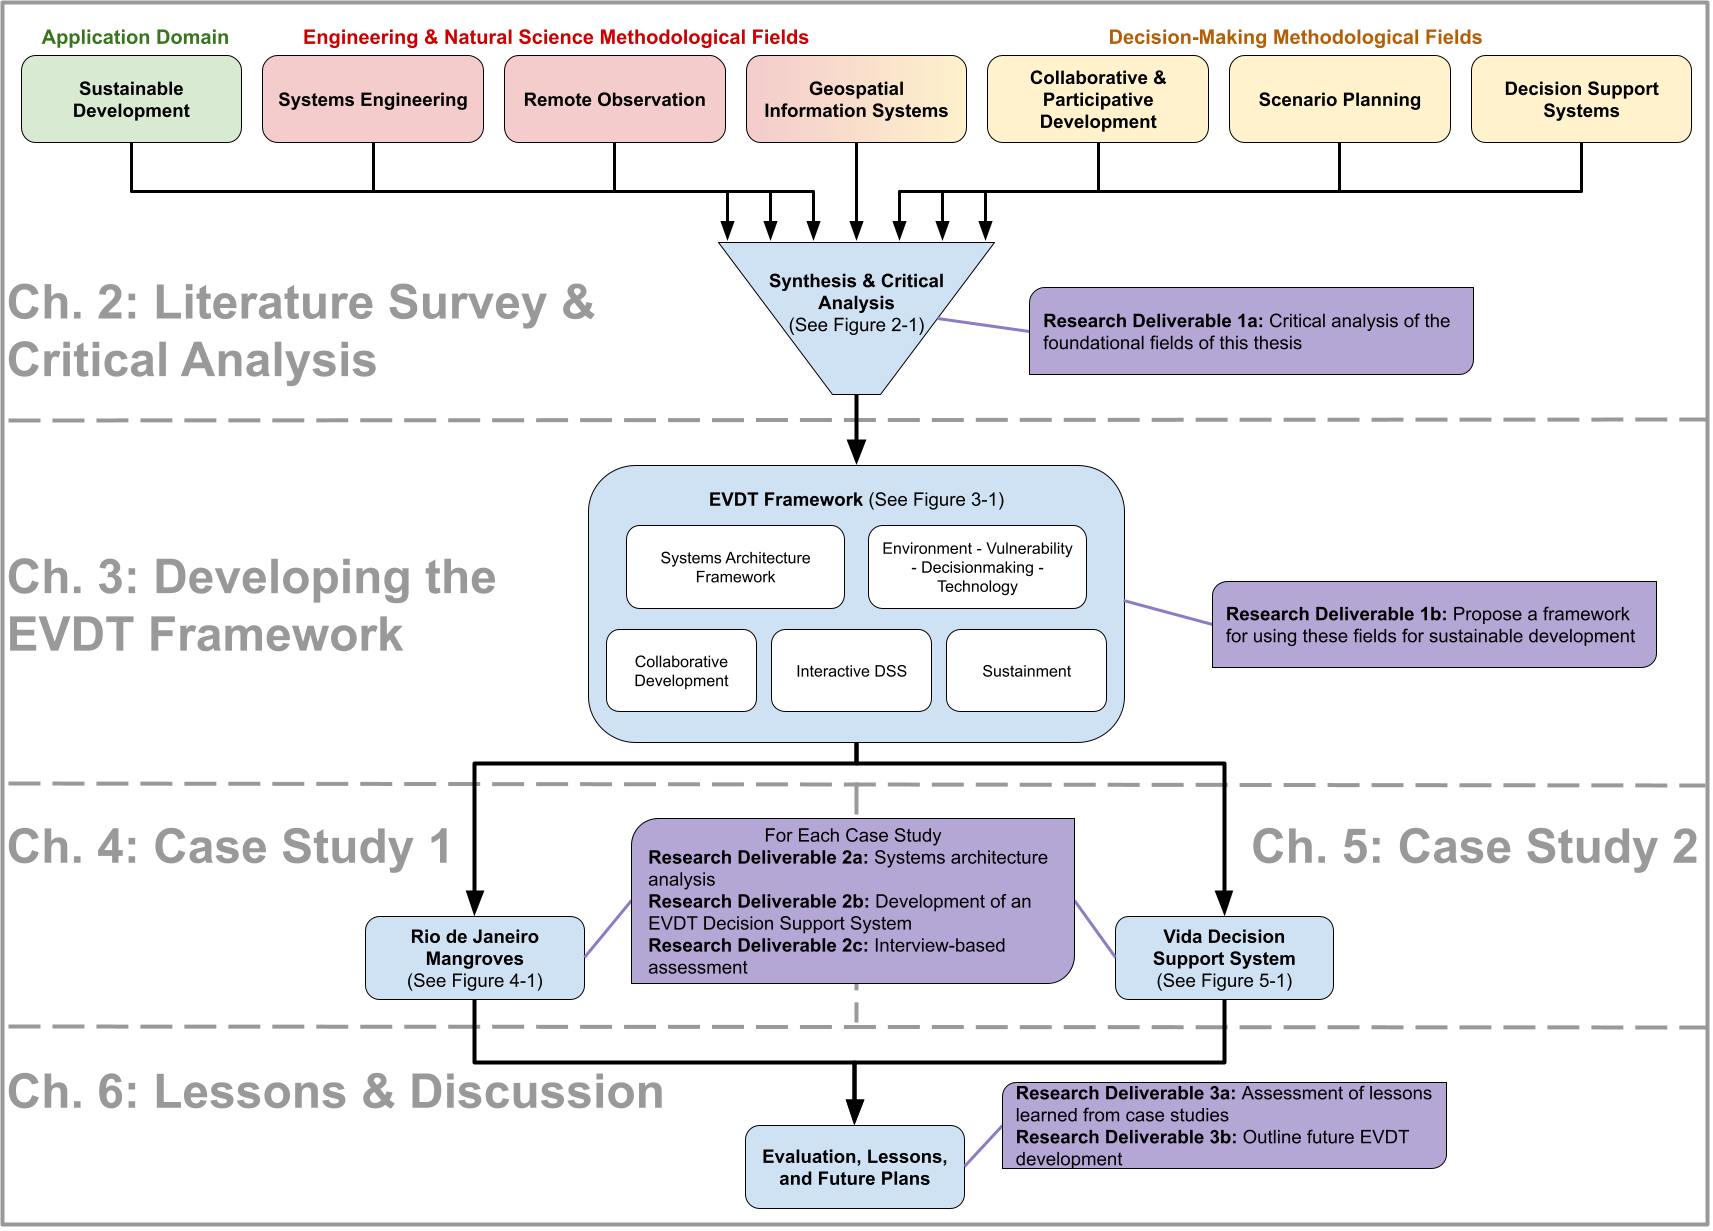
\includegraphics[scale=0.3]{Figures/chap1/structure.png}
	\caption[Thesis Structure]{Thesis Structure}
	\label{fig:structure}
\end{figure}
\end{landscape}
 

\section{\hlc[red]{Intended Audiences For This Thesis}}

[those interested in applied modeling / science]

[those interested in sustainable development]

[those interested in earth observation - space]

[those interested in environment]